\section{Decoder}

The decoder module is a crucial component in the control unit of a processor, responsible for interpreting 32-bit instructions and generating control signals that manage the processor's operations.
The inputs to the decoder module include a 32-bit instruction and a 64-bit program counter (pc). The instruction to be decoded comprises the opcode, function codes, and operand addresses, while the program counter indicates the address of the instruction. The outputs of the decoder include several control signals (\texttt{branch}, \texttt{memRead}, \texttt{memWrite}, \texttt{memToReg}, \texttt{aluSrc}, \texttt{writeReg}), ALU control signals (\texttt{aluOp}, \texttt{aluCtl}), register addresses (\texttt{readAddr01}, \texttt{readAddr02}, \texttt{writeAddr01}), the updated program counter (\texttt{newPC}, \texttt{curretPC}), and a 64-bit immediate value (\texttt{immidiateValue}).

\subsection{Truth Table}
The truth table below summarizes the control signals generated by the decoder module for each instruction type.
\setlength{\tabcolsep}{6pt} % Adjust as necessary
\begin{table}[h]
\centering
\setlength{\tabcolsep}{4pt} % Adjust as necessary
\begin{tabularx}{\textwidth}{|p{2.4cm}|p{2cm}|p{2cm}|X|X|X|X|X|X|}
\hline
\textbf{Instruction} & \textbf{ALUSrc} & \textbf{Mem to}\newline \textbf{Reg} & \textbf{Reg} \newline \textbf{Write} & \textbf{Mem} \newline \textbf{Read} & \textbf{Mem} \newline \textbf{Write} & \textbf{Branch} & \textbf{ALU} \newlinw \textbf{Op1} & \textbf{ALU} \newlinw \textbf{Op0} \\
\hline
R-format & 0 & 0 & 1 & 0 & 0 & 0 & 1 & 0 \\
\hline
ld & 1 & 1 & 1 & 1 & 0 & 0 & 0 & 0 \\
\hline
sd & 1 & X & 0 & 0 & 1 & 0 & 0 & 0 \\
\hline
beq & 0 & X & 0 & 0 & 0 & 1 & 0 & 1 \\
\hline
\end{tabularx}
\caption{Setting of the control lines is completely determined by the opcode fields of the
instruction.}
\end{table}

\subsection{Instruction Types}
The decoder module handles four instruction types: R-Type, Memory Load, Memory Store, and Branch instructions.

\textbf{R-Type Instructions}
R-Type instructions perform arithmetic and logical operations between registers. The control signals generated for R-Type instructions indicate no branching or memory access, with the ALU using register operands and writing back to the register file. Examples of R-Type instructions include ADD, SUB, AND, and OR. The ALU operations for R-Type instructions are specified by \texttt{aluOp} and \texttt{aluCtl} based on the function codes.

\textbf{Memory Load Instructions}
Memory Load instructions load data from memory into a register. The control signals for these instructions enable memory read, with the ALU performing address calculation and the data being written back to the register. An example of a Memory Load instruction is LW (load word). The immediate value for Memory Load instructions is extracted and sign-extended from the instruction.

\textbf{Memory Store Instructions}
Memory Store instructions store data from a register into memory. The control signals for these instructions enable memory write, with the ALU performing address calculation and no register write back. An example of a Memory Store instruction is SW (store word). The immediate value for Memory Store instructions is extracted from the instruction and combined into two parts.

\textbf{Branch Instructions}
Branch instructions perform conditional jumps based on register comparisons. The control signals for these instructions enable branching, with the ALU performing subtraction to compare register values. An example of a Branch instruction is BEQ (branch if equal). The immediate value for Branch instructions is extracted and sign-extended from the instruction.

\textbf{Control Signal Generation}
Control signals are generated based on the instruction's opcode. For R-Type instructions, the signals are set for arithmetic or logical operations with register operands. For Memory Load instructions, the signals enable memory read and data transfer to a register. For Memory Store instructions, the signals enable memory write from a register. For Branch instructions, the signals configure the ALU for comparison and enable branching. The ALU control signals (\texttt{aluOp} and \texttt{aluCtl}) are derived from the opcode and function codes. For R-Type instructions, ALU control is based on \texttt{funct7} and \texttt{funct3}. For Memory Load and Store instructions, the ALU is set to perform address calculation (addition). For Branch instructions, the ALU is set to perform subtraction for comparison.

\textbf{Immediate Value Extraction}
Immediate values are extracted and sign-extended to 64 bits for memory access and branch instructions, facilitating address calculation or branch target computation. This process ensures that the instructions are accurately interpreted and executed by the processor.


\subsection{Decoder Functioning}


\begin{itemize}
    \item The decoder module is responsible for interpreting the instruction and generating control signals for other components within a CPU. This functionality is depicted in the block diagram.
    \item \textbf{Instruction Fetch:} The 32-bit instruction, fetched from memory, serves as the input that needs to be decoded.
    \item \textbf{Program Counter (PC):} Holds the current address of the instruction being executed.
    \item \textbf{Opcode Decoder:} Extracts the opcode from the instruction to determine the type of instruction and generate the appropriate control signals.
     \item \textbf{Function Decoder:} Extracts the function codes (\texttt{funct7} and \texttt{funct3}) from the instruction to specify the particular operation (e.g., ADD, SUBTRACT, AND, OR) for R-type instructions.
    
\begin{figure}[H]
    \centering
    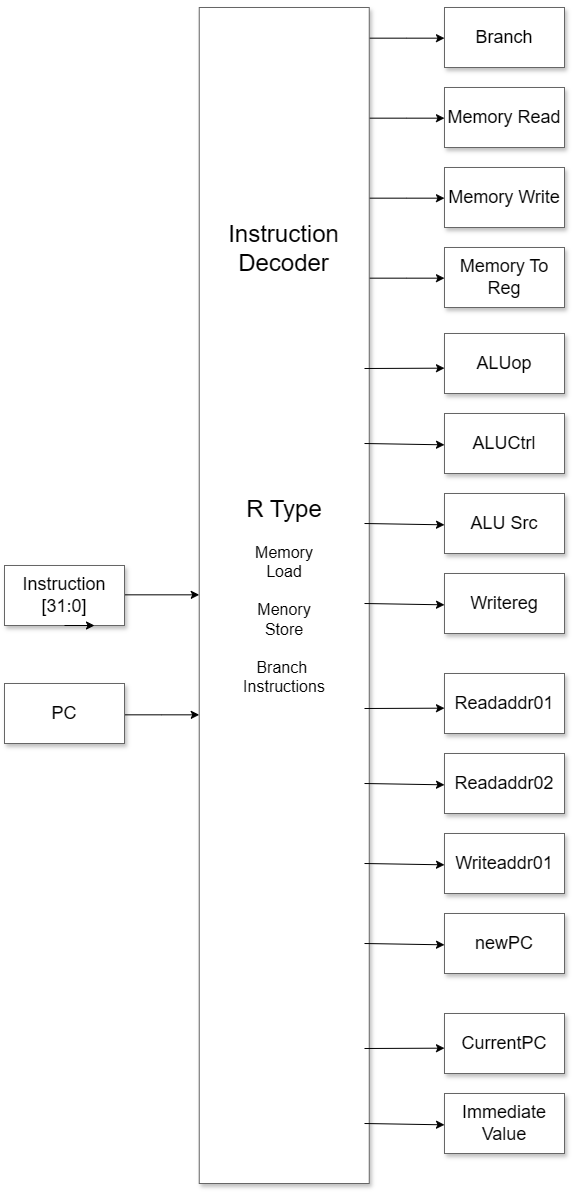
\includegraphics[width=0.95\textwidth, height=0.8\textheight]{Image/Decoder Block Diagram.drawio.png}
    \caption{Instruction Decoder}
    \label{fig: Instruction Decoder}
\end{figure}

   
    \item \textbf{Read Address 1 (rs1) and Read Address 2 (rs2):} Extract the respective fields from the instruction, specifying the source registers for the operation.
    \item \textbf{Write Address (rd):} Extracts the field indicating the destination register for the operation's result.
    \item \textbf{Immediate Value Extraction:} Handles the extraction of immediate values from the instruction for relevant operations.
    \item \textbf{Current PC:} Represents the address of the current instruction.
    \item \textbf{New PC:} Incremented by 4, points to the next instruction.
    \item \textbf{Control Unit:} Generates control signals based on the opcode, including signals for Branch, MemRead, MemWrite, MemToReg, ALUSrc, and WriteReg.
    \item \textbf{ALU Control Unit:} Produces ALU control signals (\texttt{ALUOp} and \texttt{ALUCtl}) derived from the opcode and function codes. Specific control signals such as Branch Control manage branching operations, Memory Read Control oversees memory read operations, Memory Write Control handles memory write operations, Memory to Register Control determines whether data from memory or the ALU is written to the register, ALU Source Control decides if the second ALU operand is a register value or an immediate value, and Write Register Control governs whether the result is written to a register.
    \item \textbf{Arithmetic Logic Unit (ALU):} Performs arithmetic or logical operations as specified by the control signals.
    \item \textbf{Register File:} Holds the CPU registers, interfacing with read and write addresses to access or store data.
    \item This comprehensive setup ensures the decoder module functions effectively, interpreting instructions and coordinating the necessary control signals for proper CPU operation.
\end{itemize}


